
% We summarize existing work with respect to time series distance metrics and representations. We then delve further into the field of metric learning and recent applications of metric learning paradigms to time series.

% ------------------------------------------------
\subsection{Hand-Crafted Distance Measures}
% ------------------------------------------------

Historically, most work on distance measures between time series has consisted of hand-crafted algorithms designed to reflect prior knowledge about the nature of time series. By far the most prevalent is the Dynamic Time Warping (DTW) distance \citep{dtw}. This is obtained by first aligning two time series using dynamic programming, and then computing the Euclidean distance between them. DTW requires time quadratic in the time series' length in the worst case, but is effectively linear time when used for similarity search; this is thanks to numerous lower bounds that allow early abandoning of the computation in almost all cases \citep{ucrSuite}.

Other handcrafted measures include the Uniform Scaling Distance \citep{originalUS}, the Scaled Warped Matching Distance \citep{swm}, the Complexity-Invariant Distance \citep{cid}, the Shotgun Distance \citep{shotgunDistance}, and many variants of DTW, such as weighted DTW \citep{weightedDTW}, DTW-A \citep{nontrivial}, and global alignment kernels \citep{gak}. However, nearly all of these measures are defined only for univariate time series, and generalizing them to multivariate time series is not trivial \citep{nontrivial}. % 1) are defined only for univariate time series, and 2) are rarely, if ever, used. Consequently, our experiments focus only on DTW.

% As a result of both this and the fact that almost all works of which we are aware employ unmodified DTW (plus its lower bounds), we only compare to DTW in our experiments.

% Because it is not clear how to effectively generalize most of these measures to multivariate time series, and almost all works of which we are aware employ unmodified DTW (plus its lower bounds), we only compare to DTW in our experiments.

% Before using any of these distances, is it common to first z-normalize the time series, so that the distances are invariant to differences in mean and variance between time series \citep{ucrSuite}.

% ------------------------------------------------
\subsection{Hand-Crafted Representations}
% ------------------------------------------------

In addition to hand-crafted functions of raw time series, there are numerous hand-crafted representations of time series. Perhaps the most common are Symbolic Aggregate Approximation (SAX) \citep{sax} and its derivatives \citep{isax2,saxVSM}. These are discretization techniques that low-pass filter, downsample, and quantize the time series so that they can be treated as strings. Slightly less lossy are Adaptive Piecewise Constant Approximation \citep{apca}, Piecewise Aggregate Approximation \citep{paa}, and related methods, which approximate time series as sequences of low-order polynomials.

% More recently, bag-of-patterns (BOP) representations have become common. These consist of inspecting subsequences of the time series for the presence of particular ``patterns''---such as mapping to particular SAX strings \citep{saxVSM}, being within a certain distance of other subsequences \citep{extract}, or having certain frequency content of a certain amplitude \citep{weasel}---and storing the counts of each pattern.

The most effective of these representations tend to be extremely complicated; the current state-of-the-art \citep{weasel}, for example, entails windowing, Fourier transformation, quantization, bigram extraction, and ANOVA F-tests, among other steps. Moreover, it is not obvious how to generalize them to multivariate time series.

% \subsection{Deep Metric Learning}

% Learning-based approaches to measuring distance between data points - in the context of images, videos, and text - have gained traction in recent years. Most work in the field of metric learning is supervised. A common objective within the field of metric learning is to learn an embedded distance such that data points of the same class exist closer to one another than data points of separate classes. This objective may be best accomplished through Siamese architecture, where multiple inputs are fed in at the same time. Thus, the network optimizes the relationship between the input points as it develops the appropriate embedding.

% ------------------------------------------------
\subsection{Metric Learning for Time Series}
% ------------------------------------------------

A promising alternative to hand-crafted representations and distance functions for time series is metric learning. This can take the form of either learning a distance function directly or learning a representation that can be used with an existing distance function.

Among the most well-known methods in the former category is that of \citep{dtwLearnedConstraints}, which uses an iterative search to learn data-dependent constraints on DTW alignments. More recently, \citet{mddtw} use a learned Mahalanobis distance to improve the accuracy of DTW. Both of these approaches yield only a pseudometric, which does not obey the triangle inequality. To come closer to a true metric, \citet{decade} combined a large-margin classification objective with a sampling step (even at test time) to create a DTW-like distance that obeys the triangle inequality with high probability as the sample size increases.

In the second category are various works that learn to embed time series into Euclidean space. \citet{siameseRecurrent} use recurrent neural networks in a Siamese architecture \citep{siameseOrig} to learn an embedding; they optimize the embeddings to have positive inner products for time series of the same class but negative inner products for those of different classes. A similar approach that does not require class labels is that of \citet{ldps}. This method trains a Siamese, single-layer CNN to embed time series in a space such that the pairwise Euclidean distances approximate the pairwise DTW distances. \citet{spiral} optimize a similar objective, but do so by sampling the pairwise distances and using matrix factorization to directly construct feature representations for the training set (i.e., with no model that could be applied to a separate test set).

% A great deal of work has been done on learning representations for the special case of speech time series \citep{speechNetsOverview}, but relatively little has been done on time series in general. The MDDTW of \citep{mddtw} uses a learned Mahalanobis distance to improve the accuracy of DTW. \citep{siameseRecurrent} use recurrent neural networks in a Siamese architecture \citep{siameseOrig} to learn an embedding; they optimize the embeddings to have positive inner products for time series of the same class but negative inner products for those of different classes. A similar approach that does not require class labels is that of \citet{ldps}. This method trains a siamese, single-layer CNN to embed time series in a space such that the pairwise Euclidean distances approximate the pairwise DTW distances. \citet{spiral} seeks to optimize much the same objective, but does so by sampling the pairwise similarities and using matrix factorization to directly construct feature representations for the training set (with no model that could be applied to a separate test set). Finally, DECADE \citep{decade} combines a large-margin classification objective with a sampling step (even at test time) to create a DTW-like distance that obeys the triangle inequality in expectation.

These methods seek to solve much the same problem as Jiffy but, as we show experimentally, produce metrics of much lower quality. % Indeed, several of them fail to outperform simple baselines using the original data.

% Often, these applications of metric learning to time series fail to fully capitalize on the information contained within shapelets. Many restrict their shapelet search to the discrete space of subsequences available in the training set, while others fail to produce a distance metric. Surprisingly, we show that similarity-based loss functions that have proven successful in facial recognition fail to serve time series as well.


% \begin{figure*}[t]
% \begin{center}
% % 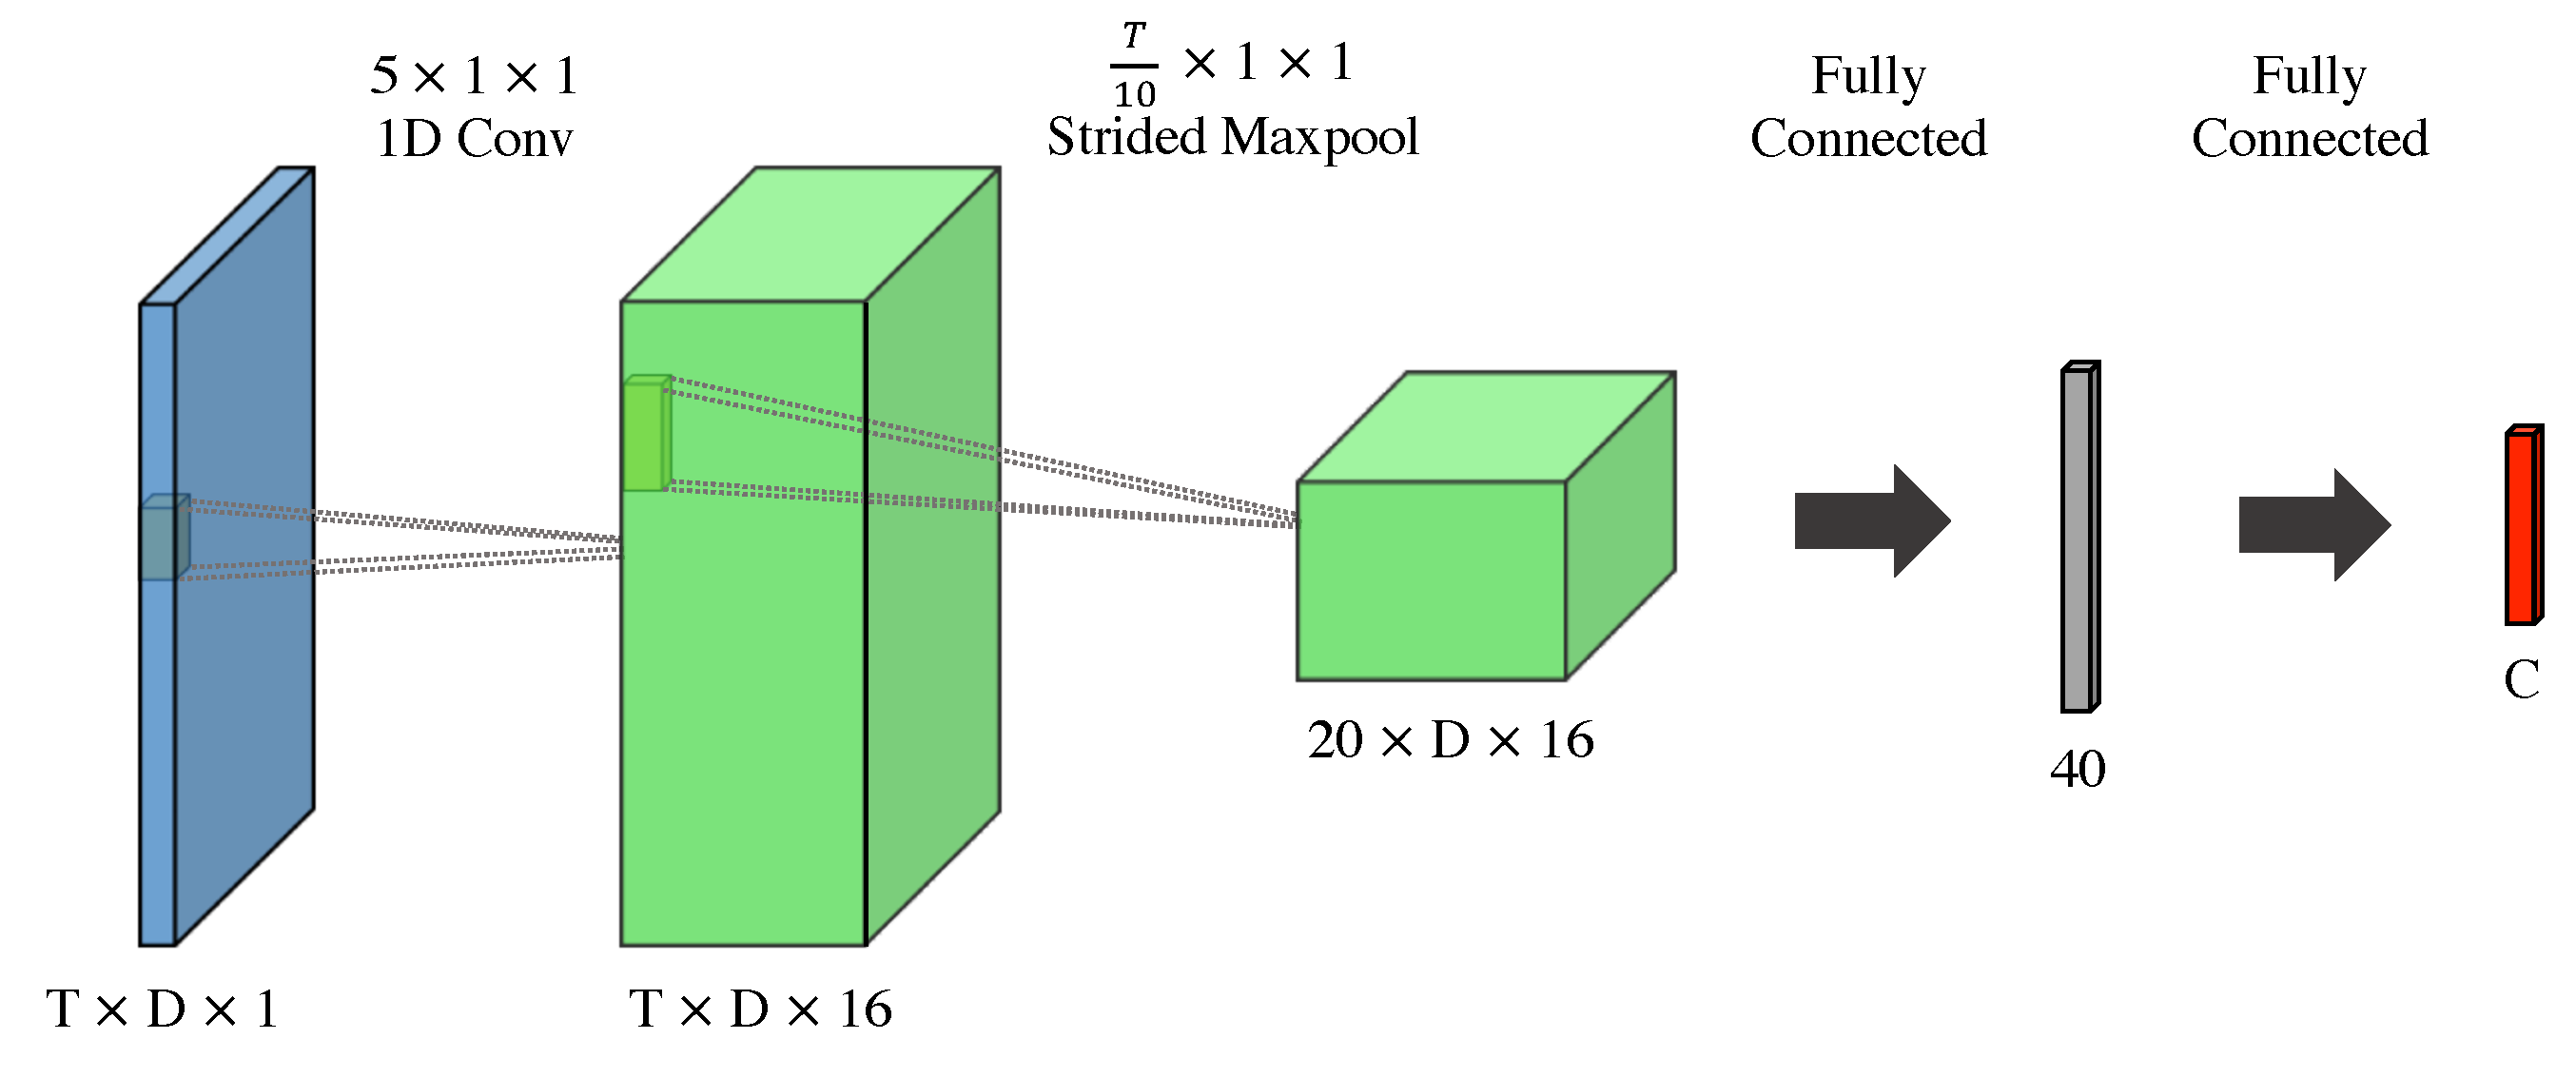
\includegraphics[width=\linewidth]{arch}
% 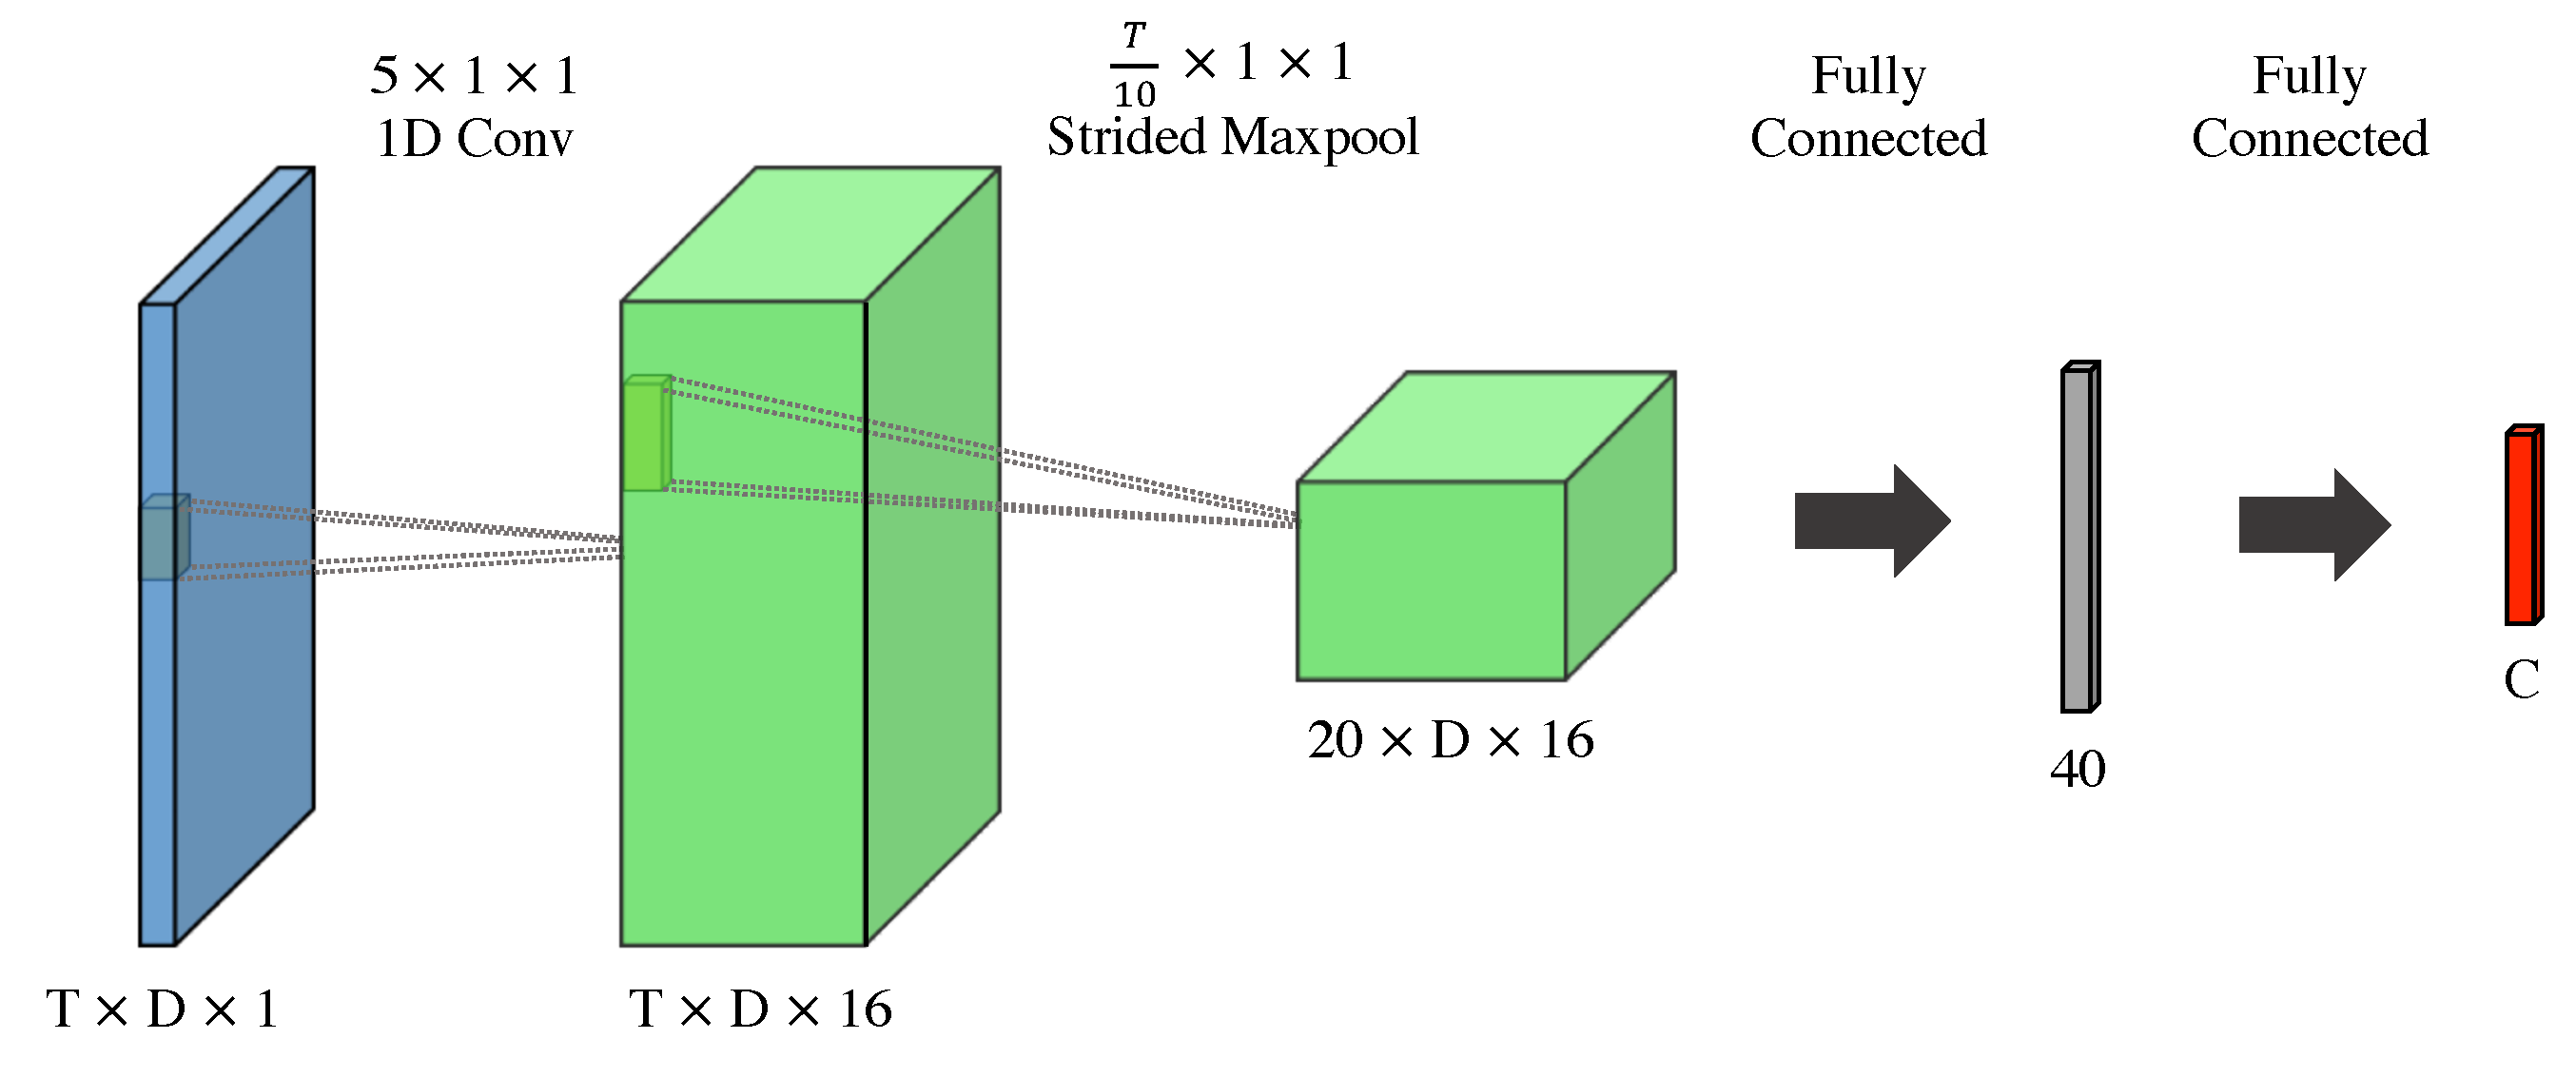
\includegraphics[width=.9\textwidth]{arch}
% % \vspace*{-2mm}
% \label{fig:arch}
% \caption{Architecture of the proposed model. TODO more explanation}
% \end{center}
% \end{figure*}

